\documentclass{beamer}

\usepackage{fontspec}
\usepackage{xeCJK}
\setCJKmainfont{DFFN_R3.TTC}
\XeTeXlinebreaklocale "zh"
\XeTeXlinebreakskip = 0pt plus 1pt
\linespread{1.3}
\allowdisplaybreaks

\newcommand{\weib}{\CJKfamily{weib}}
\newcommand{\hkss}{\CJKfamily{hkss}}
\newcommand{\hksy}{\CJKfamily{hksy}}
\newcommand{\lth}{\CJKfamily{lth}}
\usepackage{color}
\usepackage{booktabs}
\usepackage{tabularx}
\usepackage{caption}
\usepackage{tikz}
\usepackage{verbatim}
\usepackage{pgfplotstable}
\pgfplotsset{width=12cm}
\pgfplotsset{height=7cm}
\pgfplotsset{compat=1.13}

\usetheme{EastLansing}
\usetikzlibrary{positioning}
\useinnertheme{rectangles}
\usefonttheme{professionalfonts}

\newcommand{\lw}{0.8mm}
\setbeamercovered{transparent}


%\AtBeginSection[]
%{
  %\begin{frame}<beamer>
	%\frametitle{報告大綱}
	%%\frametitle{RoadMap}
    %\tableofcontents[currentsection]
  %\end{frame}
%}

\title{Paper Report}
\subtitle{\textcolor[rgb]{0.00,0.50,1.00}{{Speech Processing \& Machine Learning Laboratory}}}
\author{徐瑞陽}
\date{2019/04/10}
\begin{document}



\begin{frame}
\maketitle
\end{frame}

\begin{frame}
  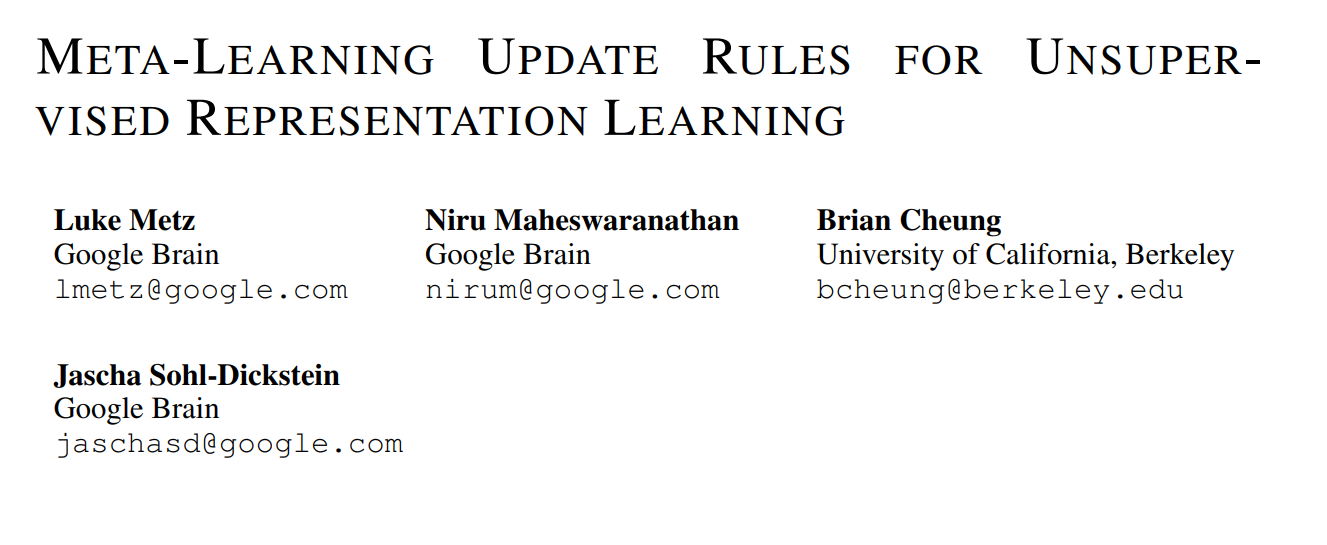
\includegraphics[width=\textwidth]{fig/title.png}
  \center ICLR 2019
  \center (8,8,8)
\end{frame}


\begin{frame}
\frametitle{Outline}
\tableofcontents
\end{frame}

\section{Survey on Meta Learning}
\subsection{Problem Formulation}
\begin{frame}{Goal}

\[ \theta^\star = \arg \max_\theta \mathbb{E}_{\mathcal{D} \sim p(\mathcal{D}) }[\mathcal{A}_\theta(\mathcal{D})]\]

$\mathcal{A}$ depends on which application we want to learn \\ 
(e.g classification, regression... and MORE!!)
\end{frame}

\begin{frame}{One Instance - Few-shot classification}

  \[ \theta^\star = \arg \max_\theta \mathbb{E}_{L \subset \mathcal{L}} \, [ \mathbb{E}_{S^L \subset \mathcal{D}, B^L \subset \mathcal{D}}[\sum_{(x,y) \in B^L} \log P_\theta(y|x,S^L)] \,  ]\]

  \begin{itemize}
    \item sample subset of label $L \subset \mathcal{L}$ to split \texttt{meta-train}, \texttt{meta-test}
    \item $S^L$ is training data in \texttt{meta-train}, also called \textit{support set}
    \item $B^L$ is testing data in \texttt{meta-train}
    \item $(S^L, B^L)$ is called \textit{task} in some literature
    \item In this case, $\mathcal{A}_\theta$ is likelihood $P_\theta(y|x)$
  \end{itemize}
\end{frame}

\subsection{Common Approaches}
\begin{frame}{Common Approaches}
  \begin{itemize}
    \item Metric-based
    \item Model-based
    \item \textbf{Optimization-based}: The paper reported today focus on
  \end{itemize}
\end{frame}

\begin{frame}{Metric-based Approach}
  What to share: \textbf{weight of feature encoder}
  \[ P_\theta (y|x,S) = \sum_{(x,x_i) \in S} k_\theta (x,x_i) y_i \]
  \begin{itemize}
    \item $k_\theta$ is kernel function to measure similarity
    %\item good feature encoder imply good $k_\theta$
    \item Implementation: via \textbf{model structure design}
      \begin{itemize}
        \item Conv. Siamse NN ($\rightarrow$ Relation Network)
        \item Matching Network
        \item Prototypical Network
      \end{itemize}
    \item As far as I know, limited application in classification only
  \end{itemize}
\end{frame}

\begin{frame}{Model-base Approach}
  What to share: \textbf{strategy of r/w memory}
  \[ P_\theta(y|x,S) = f_\theta(x,S) \]
  \begin{itemize}
    \item Retrieve experiences learnt in support set to answer
    \item Implementation: via external memory (e.g NTM), fusing $S$ (e.g convolution)
    \begin{itemize}
      \item NTM-based: MANN (LRUA, surprise-based)
      \item Temporal Convolution: SNAIL (pretty brutal... )
    \end{itemize}
  \end{itemize}
\end{frame}

\begin{frame}{Optimization-based Approach}
  What to share: optimizer, initial weight, hyper-param, \textbf{update rule}...
  \begin{itemize}
    \item initial weight: MAML and its variant\\
      (PMAML, FOMAML $\rightarrow$ Reptile)
    \item optimizer: LSTM Meta-Learner
    \item update rule: Today's paper
  \end{itemize}
\end{frame}

\subsection{Applications}

\begin{frame}{Applications}
  \begin{itemize}
    \item Few-shot classification
    \item Reinforcement Learning
    \item Generative modeling: NMT (EMNLP 2018), TTS (ICLR 2019)
    \item \textbf{Unsupervised Representation Learning}
  \end{itemize}
\end{frame}

\begin{frame}{Desirable Properties}
  Quote from Chelsea Finn's thesis
  \begin{itemize}
    \item Expressive power to represent ``learning algorithm''
    \item Generalization power
    \item Ambuiguity modeling power: what \textbf{P}MAML did
  \end{itemize}
\end{frame}


\section{Meta-Learning Update Rules For Unsupervised Learning}
\begin{frame}
  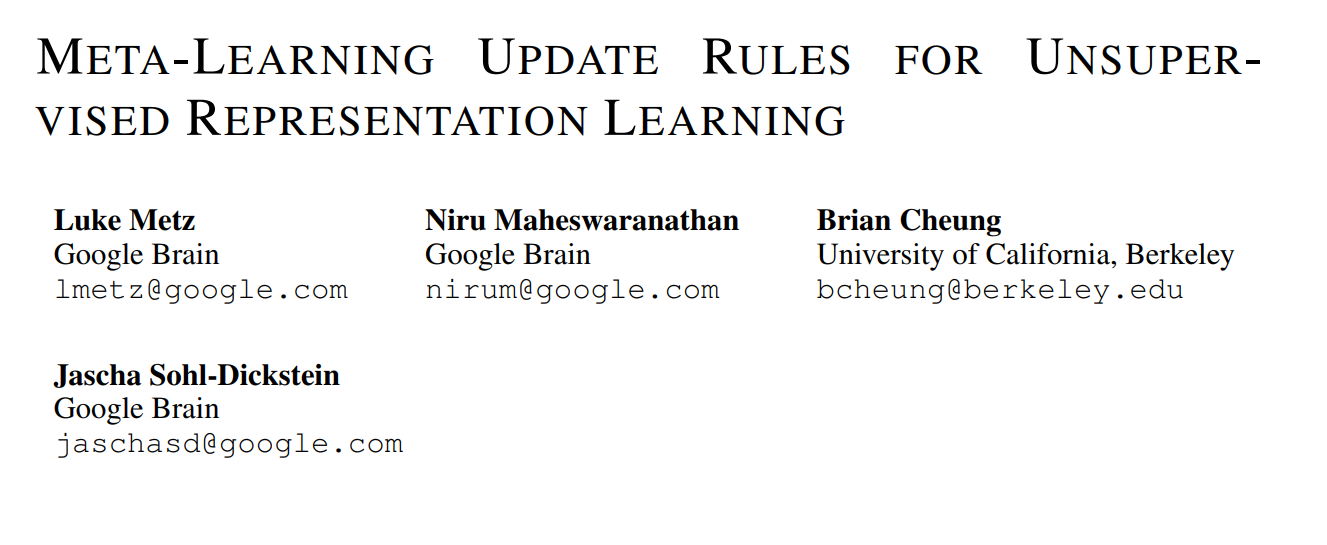
\includegraphics[width=\textwidth]{fig/title.png}
  \center ICLR 2019
\end{frame}

\begin{frame}{Motivation}
\end{frame}

\begin{frame}{Flow}
\end{frame}

\begin{frame}{Experiments}
\end{frame}

\section{Comparison}
\subsection{Unsupervised Learning via Meta-Learning}

\begin{frame}
  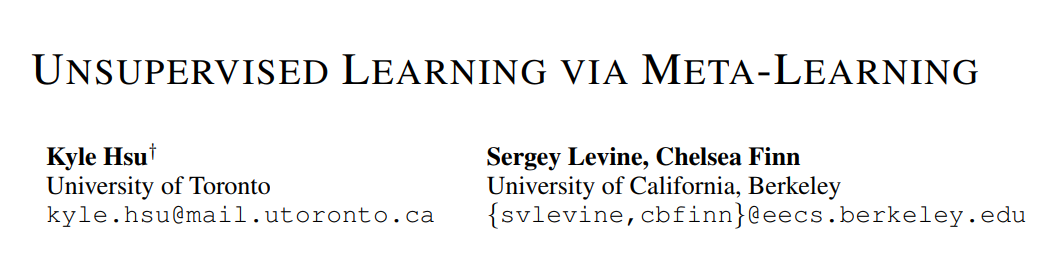
\includegraphics[width=\textwidth]{fig/ULML.png}
  \center ICLR 2019
\end{frame}

\subsection{LSTM Meta-Learner}
\begin{frame}
  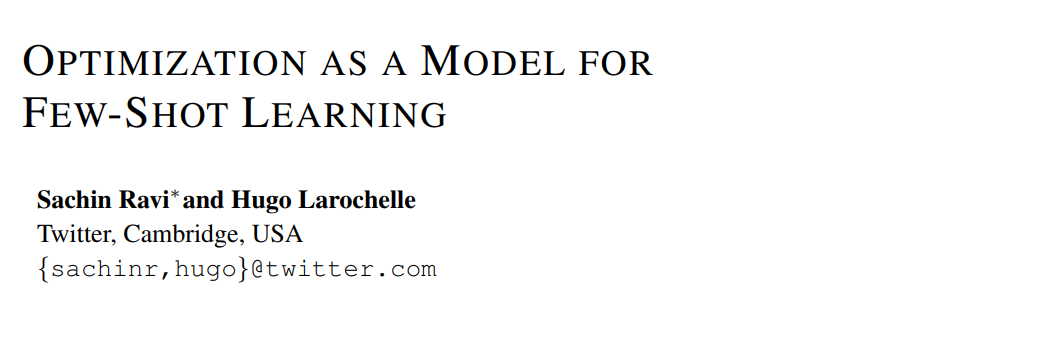
\includegraphics[width=\textwidth]{fig/LSTM-Meta-Learner.png}
  \center ICLR 2017
\end{frame}

\section{Future Work}

\section{MISC}
\begin{frame}
	\begin{center}
    %\weib{\LARGE{謝謝聆聽!}}
    \LARGE{Questions?}
	\end{center}
\end{frame}


\subsection{Appendix}
\end{document} 
